\documentclass[crop,tikz]{standalone}
\usepackage{tikz}
\usepackage{xcolor}
\usetikzlibrary{backgrounds,calc,shapes,arrows,decorations.pathreplacing,decorations.markings,patterns,positioning,3d,fit,shapes.geometric}

% Define colors
\definecolor{edgecolor}{RGB}{64, 64, 140}
\definecolor{nodecolor}{RGB}{180, 60, 60}
\definecolor{fillcolor1}{RGB}{250, 230, 200}
\definecolor{fillcolor2}{RGB}{220, 240, 220}
\definecolor{fillcolor3}{RGB}{200, 220, 250}
\definecolor{fillcolor4}{RGB}{240, 220, 240}
\definecolor{opefill}{RGB}{245, 230, 210}

\begin{document}
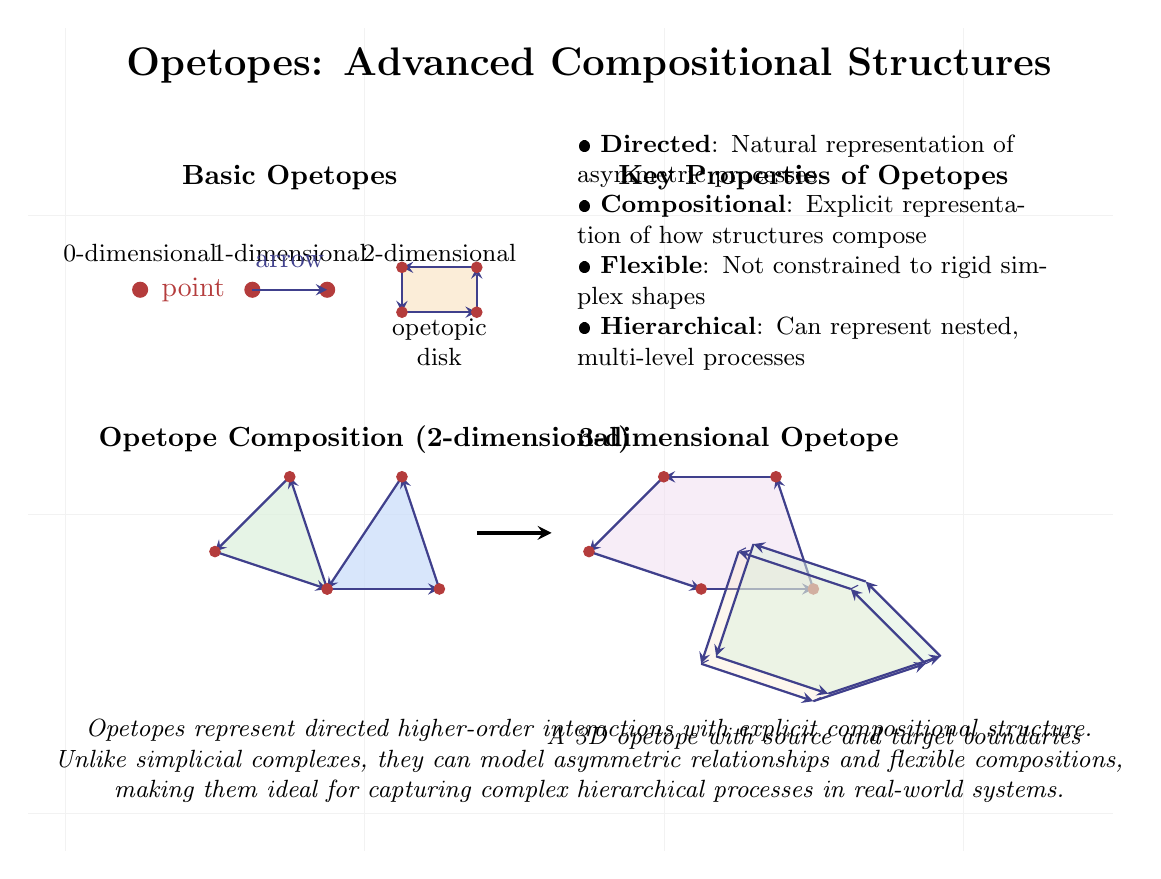
\begin{tikzpicture}[scale=0.95]
  % Grid for organization
  \draw[step=4cm, black!5, very thin] (-0.5,-0.5) grid (14,10.5);
  
  % Title
  \node[font=\Large\bfseries] at (7,10) {Opetopes: Advanced Compositional Structures};
  
  % 0D and 1D Opetopes 
  \node[font=\bfseries] at (3,8.5) {Basic Opetopes};
  
  % 0D opetope (point)
  \node[font=\bfseries, font=\small] at (1,7.5) {0-dimensional};
  \filldraw[nodecolor] (1,7) circle (0.1) node[right=0.15cm] {point};
  
  % 1D opetope (arrow)
  \node[font=\bfseries, font=\small] at (3,7.5) {1-dimensional};
  \filldraw[nodecolor] (2.5,7) circle (0.1);
  \filldraw[nodecolor] (3.5,7) circle (0.1);
  \draw[->, >=stealth, thick, edgecolor] (2.5,7) -- (3.5,7) node[midway, above=0.15cm] {arrow};
  
  % 2D opetope (disk/polygon)
  \node[font=\bfseries, font=\small] at (5,7.5) {2-dimensional};
  
  \coordinate (A1) at (4.5,6.7);
  \coordinate (B1) at (5.5,6.7);
  \coordinate (C1) at (5.5,7.3);
  \coordinate (D1) at (4.5,7.3);
  
  % Draw the 2D opetope as a filled region with directed boundary
  \filldraw[fillcolor1, opacity=0.7] (A1) -- (B1) -- (C1) -- (D1) -- cycle;
  
  % Arrows for boundary
  \draw[->, >=stealth, thick, edgecolor] (A1) -- (B1);
  \draw[->, >=stealth, thick, edgecolor] (B1) -- (C1);
  \draw[->, >=stealth, thick, edgecolor] (C1) -- (D1);
  \draw[->, >=stealth, thick, edgecolor] (D1) -- (A1);
  
  % Vertices
  \filldraw[nodecolor] (A1) circle (0.07);
  \filldraw[nodecolor] (B1) circle (0.07);
  \filldraw[nodecolor] (C1) circle (0.07);
  \filldraw[nodecolor] (D1) circle (0.07);
  
  \node[align=center, font=\small] at (5,6.3) {opetopic\\disk};
  
  % Higher-dimensional opetope explanation
  \node[font=\bfseries] at (10,8.5) {Key Properties of Opetopes};
  
  \node[align=left, font=\small, text width=6cm] at (10,7.5) {
    \textbf{• Directed}: Natural representation of asymmetric processes\\
    \textbf{• Compositional}: Explicit representation of how structures compose\\
    \textbf{• Flexible}: Not constrained to rigid simplex shapes\\
    \textbf{• Hierarchical}: Can represent nested, multi-level processes
  };
  
  % 2D Opetope Composition
  \node[font=\bfseries] at (4,5) {Opetope Composition (2-dimensional)};
  
  % Draw the first opetope
  \coordinate (P1) at (2,3.5);
  \coordinate (P2) at (3.5,3);
  \coordinate (P3) at (3,4.5);
  
  \filldraw[fillcolor2, opacity=0.7] (P1) -- (P2) -- (P3) -- cycle;
  \draw[->, >=stealth, thick, edgecolor] (P1) -- (P2);
  \draw[->, >=stealth, thick, edgecolor] (P2) -- (P3);
  \draw[->, >=stealth, thick, edgecolor] (P3) -- (P1);
  \filldraw[nodecolor] (P1) circle (0.07);
  \filldraw[nodecolor] (P2) circle (0.07);
  \filldraw[nodecolor] (P3) circle (0.07);
  
  % Draw the second opetope
  \coordinate (Q1) at (3.5,3);
  \coordinate (Q2) at (5,3);
  \coordinate (Q3) at (4.5,4.5);
  
  \filldraw[fillcolor3, opacity=0.7] (Q1) -- (Q2) -- (Q3) -- cycle;
  \draw[->, >=stealth, thick, edgecolor] (Q1) -- (Q2);
  \draw[->, >=stealth, thick, edgecolor] (Q2) -- (Q3);
  \draw[->, >=stealth, thick, edgecolor] (Q3) -- (Q1);
  \filldraw[nodecolor] (Q1) circle (0.07);
  \filldraw[nodecolor] (Q2) circle (0.07);
  \filldraw[nodecolor] (Q3) circle (0.07);
  
  % Composition arrow
  \draw[->, >=stealth, very thick] (5.5,3.75) -- (6.5,3.75);
  
  % The composite opetope
  \coordinate (R1) at (7,3.5);
  \coordinate (R2) at (8.5,3);
  \coordinate (R3) at (10,3);
  \coordinate (R4) at (9.5,4.5);
  \coordinate (R5) at (8,4.5);
  
  \filldraw[fillcolor4, opacity=0.5] (R1) -- (R2) -- (R3) -- (R4) -- (R5) -- cycle;
  \draw[->, >=stealth, thick, edgecolor] (R1) -- (R2);
  \draw[->, >=stealth, thick, edgecolor] (R2) -- (R3);
  \draw[->, >=stealth, thick, edgecolor] (R3) -- (R4);
  \draw[->, >=stealth, thick, edgecolor] (R4) -- (R5);
  \draw[->, >=stealth, thick, edgecolor] (R5) -- (R1);
  \filldraw[nodecolor] (R1) circle (0.07);
  \filldraw[nodecolor] (R2) circle (0.07);
  \filldraw[nodecolor] (R3) circle (0.07);
  \filldraw[nodecolor] (R4) circle (0.07);
  \filldraw[nodecolor] (R5) circle (0.07);
  
  % 3D Opetope Visualization
  \node[font=\bfseries] at (9,5) {3-dimensional Opetope};
  
  % Source boundary (multiple 2D opetopes arranged in a tree)
  \coordinate (S1) at (8.5,2);
  \coordinate (S2) at (10,1.5);
  \coordinate (S3) at (11.5,2);
  \coordinate (S4) at (10.5,3);
  \coordinate (S5) at (9,3.5);
  
  % Draw a 3D-like structure with multiple 2D faces
  % Back face
  \filldraw[fillcolor1, opacity=0.3] (S1) -- (S2) -- (S3) -- (S4) -- (S5) -- cycle;
  
  % Front face with slight offset for 3D effect
  \coordinate (T1) at ($(S1) + (0.2,0.1)$);
  \coordinate (T2) at ($(S2) + (0.2,0.1)$);
  \coordinate (T3) at ($(S3) + (0.2,0.1)$);
  \coordinate (T4) at ($(S4) + (0.2,0.1)$);
  \coordinate (T5) at ($(S5) + (0.2,0.1)$);
  
  \filldraw[fillcolor2, opacity=0.5] (T1) -- (T2) -- (T3) -- (T4) -- (T5) -- cycle;
  
  % Connect corresponding vertices with edges
  \draw[dashed, edgecolor] (S1) -- (T1);
  \draw[dashed, edgecolor] (S2) -- (T2);
  \draw[dashed, edgecolor] (S3) -- (T3);
  \draw[dashed, edgecolor] (S4) -- (T4);
  \draw[dashed, edgecolor] (S5) -- (T5);
  
  % Draw source boundary
  \draw[->, >=stealth, thick, edgecolor] (S1) -- (S2);
  \draw[->, >=stealth, thick, edgecolor] (S2) -- (S3);
  \draw[->, >=stealth, thick, edgecolor] (S3) -- (S4);
  \draw[->, >=stealth, thick, edgecolor] (S4) -- (S5);
  \draw[->, >=stealth, thick, edgecolor] (S5) -- (S1);
  
  % Draw target boundary
  \draw[->, >=stealth, thick, edgecolor] (T1) -- (T2);
  \draw[->, >=stealth, thick, edgecolor] (T2) -- (T3);
  \draw[->, >=stealth, thick, edgecolor] (T3) -- (T4);
  \draw[->, >=stealth, thick, edgecolor] (T4) -- (T5);
  \draw[->, >=stealth, thick, edgecolor] (T5) -- (T1);
  
  % Label the source and target
  \node[align=center, font=\small\itshape] at (10,1) {A 3D opetope with source and target boundaries};
  
  % Annotations
  \node[align=center, font=\small\itshape] at (7,0.7) {
  Opetopes represent directed higher-order interactions with explicit compositional structure.\\
  Unlike simplicial complexes, they can model asymmetric relationships and flexible compositions,\\
  making them ideal for capturing complex hierarchical processes in real-world systems.
  };
\end{tikzpicture}
\end{document}